\documentclass[12pt, twoside]{article}
\usepackage{amsmath}
\usepackage{amssymb}
\usepackage{graphicx}
\usepackage{enumerate}
\usepackage{geometry}
\usepackage{pgfplots}
\pgfplotsset{compat=1.18}
\usepackage{tikz}
\geometry{margin=1in}

\begin{document}

\begin{center}
\Large{\textbf{IB Mathematics Standard Level}} \\
\large{\textbf{Paper 1}} \\
\normalsize{12 November 2018 -- No Calculator} \\
\normalsize{90 marks total}
\end{center}

\vspace{0.5cm}

\section*{Section A}

\begin{enumerate}

% Question 1 [6 marks]
\item \textbf{[6 marks]} The following diagram shows a circle with centre A and radius 6\,cm.

\begin{center}
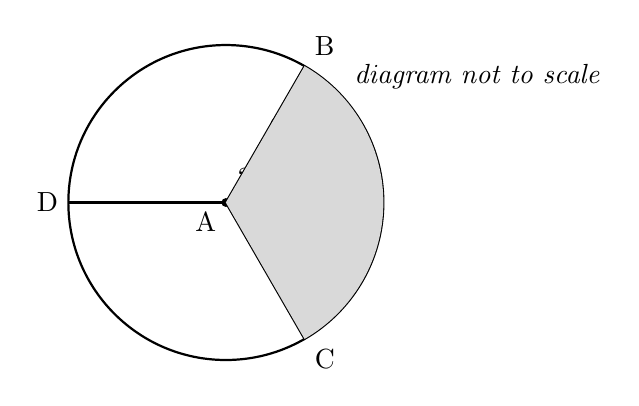
\begin{tikzpicture}[scale=0.8]
    % Draw circle
    \draw[thick] (0,0) circle (2.5);
    % Draw center point A
    \fill (0,0) circle (2pt) node[below left] {A};
    % Draw radii
    \draw[thick] (0,0) -- (60:2.5) node[above right] {B};
    \draw[thick] (0,0) -- (-60:2.5) node[below right] {C};
    \draw[thick] (0,0) -- (180:2.5) node[left] {D};
    % Draw arc for angle
    \draw (0.5,0) arc (0:60:0.5);
    \node at (0.3,0.4) {2};
    % Label radius
    \node at (0.8,1.2) {6};
    % Shade the sector BAC
    \fill[gray!30] (0,0) -- (60:2.5) arc (60:-60:2.5) -- cycle;
    % Note
    \node at (4,2) {\textit{diagram not to scale}};
\end{tikzpicture}
\end{center}

The points B, C, and D lie on the circle, and $\mathrm{B\hat{A}C} = 2$ radians.

\begin{enumerate}[(a)]
    \item Find the area of the shaded sector.
    \item Find the perimeter of the non-shaded sector ABDC.
\end{enumerate}

\vspace{1cm}

% Question 2 [5 marks]
\item \textbf{[5 marks]} Two functions, $f$ and $g$, are defined in the following table.

\begin{center}
\begin{tabular}{|c|c|c|c|c|}
\hline
$x$ & $-2$ & $1$ & $3$ & $6$ \\
\hline
$f(x)$ & $6$ & $3$ & $1$ & $-2$ \\
\hline
$g(x)$ & $-7$ & $-2$ & $5$ & $9$ \\
\hline
\end{tabular}
\end{center}

\begin{enumerate}[(a)]
    \item Write down the value of $f(1)$.
    \item Find the value of $(g \circ f)(1)$.
    \item Find the value of $g^{-1}(-2)$.
\end{enumerate}

\vspace{1cm}

% Question 3 [6 marks]
\item \textbf{[6 marks]} In an arithmetic sequence, $u_1 = -5$ and $d = 3$.

\begin{enumerate}[(a)]
    \item Find $u_8$.
    \item Find the value of $n$ for which $u_n = 67$.
\end{enumerate}

\vspace{1cm}

% Question 4 [6 marks]
\item \textbf{[6 marks]} Let $b = \log_2 a$, where $a > 0$. Write down each of the following expressions in terms of $b$.

\begin{enumerate}[(a)]
    \item $\log_2 a^3$
    \item $\log_2 8a$
    \item $\log_8 a$
\end{enumerate}

\vspace{1cm}

% Question 5 [6 marks]
\item \textbf{[6 marks]} Consider the vectors $\mathbf{a} = \begin{pmatrix} 3 \\ 2p \end{pmatrix}$ and $\mathbf{b} = \begin{pmatrix} p+1 \\ 8 \end{pmatrix}$.

Find the possible values of $p$ for which $\mathbf{a}$ and $\mathbf{b}$ are parallel.

\vspace{1cm}

% Question 6 [8 marks]
\item \textbf{[8 marks]} Let $f(x) = \dfrac{6-2x}{\sqrt{16+6x-x^2}}$. The following diagram shows part of the graph of $f$.

\begin{center}
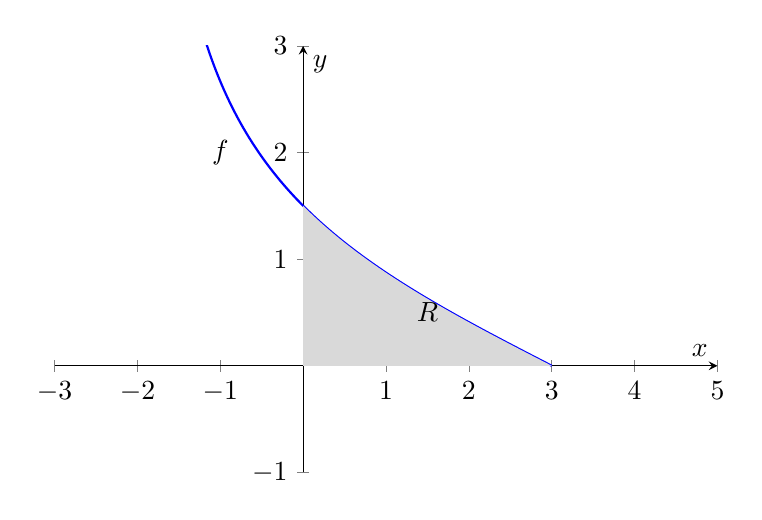
\begin{tikzpicture}
\begin{axis}[
    width=10cm,
    height=7cm,
    axis lines=middle,
    xlabel={$x$},
    ylabel={$y$},
    xmin=-3, xmax=5,
    ymin=-1, ymax=3,
    samples=200,
    smooth,
]
% f(x) = (6-2x)/sqrt(16+6x-x^2)
% Domain: 16+6x-x^2 > 0, roots at x = -2 and x = 8
\addplot[domain=-1.9:3, blue, thick] {(6-2*x)/sqrt(16+6*x-x^2)};
\node at (axis cs: -1,2) {$f$};
% Shade region R
\fill[gray!30] (axis cs:0,0) -- plot[domain=0:3, samples=100] (\x, {(6-2*\x)/sqrt(16+6*\x-\x^2)}) -- (axis cs:3,0) -- cycle;
\node at (axis cs: 1.5,0.5) {$R$};
\end{axis}
\end{tikzpicture}
\end{center}

The region $R$ is enclosed by the graph of $f$, the $x$-axis, and the $y$-axis. Find the area of $R$.

\vspace{1cm}

% Question 7 [6 marks]
\item \textbf{[6 marks]} Given that $\sin x = \dfrac{1}{3}$, where $0 < x < \dfrac{\pi}{2}$, find the value of $\cos 4x$.

\newpage

\section*{Section B}

\setcounter{enumi}{7}

% Question 8 [16 marks]
\item \textbf{[16 marks]} Let $f(x) = x^2 - 4x - 5$. The following diagram shows part of the graph of $f$.

\begin{center}
\begin{tikzpicture}
\begin{axis}[
    width=10cm,
    height=8cm,
    axis lines=middle,
    xlabel={$x$},
    ylabel={$y$},
    xmin=-3, xmax=7,
    ymin=-12, ymax=8,
    xtick={-2,-1,0,1,2,3,4,5,6},
    ytick={-10,-8,-6,-4,-2,0,2,4,6},
    samples=100,
    smooth,
]
\addplot[domain=-2:6.5, blue, thick] {x^2 - 4*x - 5};
\node at (axis cs: 5.5,4) {$f$};
\end{axis}
\end{tikzpicture}
\end{center}

\begin{enumerate}[(a)]
    \item Find the $x$-intercepts of the graph of $f$.
    \item Find the equation of the axis of symmetry of the graph of $f$.
    \item The function can be written in the form $f(x) = (x-h)^2 + k$.
    \begin{enumerate}[(i)]
        \item Write down the value of $h$.
        \item Find the value of $k$.
    \end{enumerate}
\end{enumerate}

The graph of a second function, $g$, is obtained by a reflection of the graph of $f$ in the $y$-axis, followed by a translation of $\begin{pmatrix} -3 \\ 6 \end{pmatrix}$.

\begin{enumerate}[(a)]
    \setcounter{enumii}{3}
    \item Find the coordinates of the vertex of the graph of $g$.
\end{enumerate}

\vspace{1cm}

% Question 9 [15 marks]
\item \textbf{[15 marks]} A bag contains $n$ marbles, two of which are blue. Hayley plays a game in which she randomly draws marbles out of the bag, one after another, without replacement. The game ends when Hayley draws a blue marble.

\begin{enumerate}[(a)]
    \item Find the probability, in terms of $n$, that the game will end on her
    \begin{enumerate}[(i)]
        \item first draw;
        \item second draw.
    \end{enumerate}
    \item Let $n = 5$. Find the probability that the game will end on her
    \begin{enumerate}[(i)]
        \item third draw;
        \item fourth draw.
    \end{enumerate}
\end{enumerate}

Hayley plays the game when $n = 5$. She pays \$20 to play and can earn money back depending on the number of draws it takes to obtain a blue marble. She earns no money back if she obtains a blue marble on her first draw. Let $M$ be the amount of money that she earns back playing the game. This information is shown in the following table.

\begin{center}
\begin{tabular}{|c|c|c|c|c|}
\hline
\textbf{Number of draws} & 1 & 2 & 3 & 4 \\
\hline
\textbf{Money earned back (\$$M$)} & 0 & 20 & $8k$ & $12k$ \\
\hline
\end{tabular}
\end{center}

\begin{enumerate}[(a)]
    \setcounter{enumii}{2}
    \item Find the value of $k$ so that this is a fair game.
\end{enumerate}

\vspace{1cm}

% Question 10 [16 marks]
\item \textbf{[16 marks]} Let $f(x) = x^3 - 2x^2 + ax + 6$. Part of the graph of $f$ is shown in the following diagram.

\begin{center}
\begin{tikzpicture}
\begin{axis}[
    width=10cm,
    height=9cm,
    axis lines=middle,
    xlabel={$x$},
    ylabel={$y$},
    xmin=-2, xmax=4,
    ymin=-8, ymax=10,
    samples=100,
    smooth,
]
% Using a = -3 for illustration (actual value to be found)
\addplot[domain=-1.5:3.5, blue, thick] {x^3 - 2*x^2 - 3*x + 6};
\node at (axis cs: 3,6) {$f$};
% Point P at y-intercept
\fill (axis cs: 0,6) circle (2pt) node[above right] {P};
% Tangent line L at P (slope = a = -3 when x=0)
\addplot[domain=-1.5:3, red, thick, dashed] {-3*x + 6};
\node at (axis cs: -1,8) {$L$};
% Point Q (local minimum)
\fill (axis cs: 1.82,-0.1) circle (2pt) node[below] {Q};
\end{axis}
\end{tikzpicture}
\end{center}

The graph of $f$ crosses the $y$-axis at the point P. The line $L$ is tangent to the graph of $f$ at P.

\begin{enumerate}[(a)]
    \item Find the coordinates of P.
    \item \begin{enumerate}[(i)]
        \item Find $f'(x)$.
        \item Hence, find the equation of $L$ in terms of $a$.
    \end{enumerate}
\end{enumerate}

The graph of $f$ has a local minimum at the point Q. The line $L$ passes through Q.

\begin{enumerate}[(a)]
    \setcounter{enumii}{2}
    \item Find the value of $a$.
\end{enumerate}

\end{enumerate}

\end{document}
